\status{started}
\chapter{MEG II and the Cockcroft–Walton}
\begin{refsection}
{\itshape This Chapter is dedicated to an in-depth description of the MEG search and the MEG II apparatus. After the description of the different subdetectors and their functionality a description of the beamlines will follow. MEG II is served by the main muon beamline, part of the PSI beamlines described in the Introduction Chapter, and a secondary proton beamline equipped with its own Cockcroft–Walton. This machine has different uses in the collaboration, which will be here discussed, and its functioning has been one of my main tasks.}

\section{MEG II}
\section{XEC}
    \subsection{Xe scintillation}
    \subsection{Xe as calorimeter}
    \subsection{Cryogenics}
    \subsection{PMTs}
    \subsection{Performances}
    \subsection{LED Calibration}
    \label{LED}

\section{Spectrometer}
    \subsection{COBRA}
    \label{MEG:COBRA}
    \subsection{CDCH}
    \subsection{TC}

\section{Trigger and DAQ}

\status{started}
\section{Beam and target}
    The beam lines at PSI were described in \ref{intro:beamlines}. 
    In particular, the beam line delivering $\mu^+$ to MEG II is the $\pi E5$ line. 
    This line is shown in  Fig. \ref{fig:pie5} and the key elements are here discussed

    \status{started}
    \subsection{$\pi e5$}
        This beam-line has actually two possible configurations: this will allow to share it between MEG II and Mu3e. 
        As already illustrated, the surface muons delivered by this beam-line are produced for the decay of the pions generated as secondary beams from the HIPA proton beam.
        On top of muons, pions, and positrons also are transported by the beam line: the rate of the different species is momentum dependent and is shown in Fig.~\ref{fig:pie5:rates}.
        The peak at \SI{29}{MeV/c} is the working point of the experiment.
        \begin{equation}
            \Delta R = a \left\{
                \left[  
                    \left( \frac{200 m_e}{M}\right)^{1/2} f \frac{E}{Mc^2}
                \right]^2 + 
                \left( 3.5\frac{\Delta p }{p}\right)^2
            \right\} ^{1/2} p^{3.5}
        \end{equation}
        The elements that makeup one of the two configurations, the "L" channel, were designed \textit{ad hoc} for MEG II.

        \begin{figure}
            \centering
            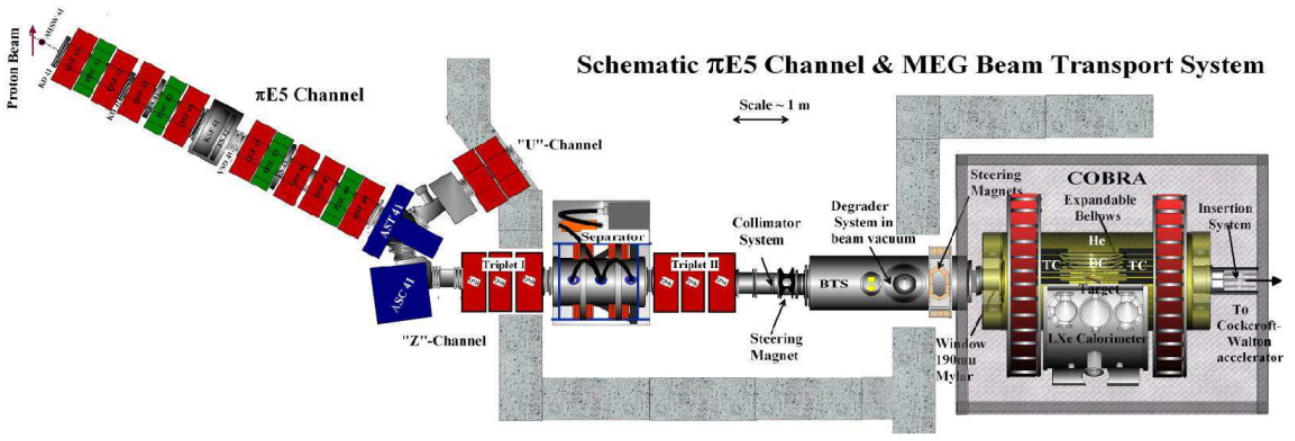
\includegraphics[width = \textwidth]{Figures/MEG/pie5_beamline.png}
            \caption{Detail of the $\pi E5$ beamline at PSI. OLD}
            \label{fig:pie5}
        \end{figure}

        \paragraph{Quadrupoles and separator}
        \paragraph{BTS}
        \paragraph{COBRA} Finally the beam enters COBRA. 
        The design choice for this element was previously illustrated (\ref{MEG:COBRA}). 
        The behavior of the beam inside this element is quite tricky to simulate consistently.
        
    \status{started}
    \subsection{Simulations}
        \paragraph{\gfb}
        \paragraph{\madx} During 2022/2023 Luca Biasia, a Master student in Pisa, developed a \madx\footnote{\madx is a general-purpose tool for charged-particle optics design and can be found \href{http://madx.web.cern.ch/madx/}{\underline{here}}.} simulation to describe the $\pi E5$ line and cross-validate the results obtained using \gfb. 
        My contribution to this simulation was only partial: I provided Luca with some working \madx examples, developed while attending the JUAS, for him to start playing with this simulation framework. 
        After this initial `starting kit', Giovanni Dal Maso has been the one overseeing the development while I only followed the updates. \\
        After a comparison with data and \gfb some discrepancies arose and, after many iterations, they were associated with the description of the fringing fields of the components in \madx. 
        The solution adopted was to slice the field maps in thin layers and define many thin `\madx elements'. 
        A comparison of the results from QSK41 to COBRA center is shown in Fig.~\ref{fig:madx_vs_g4b}
        During the beam tuning in June 2023, this simulation was crosschecked: after measuring the beam spot at COBRA center the currents of the magnets were chosen with \madx to obtain a different beam shape. 
        The measurement was consistent with the resulting simulation.
        Moving forward this tool is going to play a key role during the beam tuning.

        \begin{figure}
            \centering
            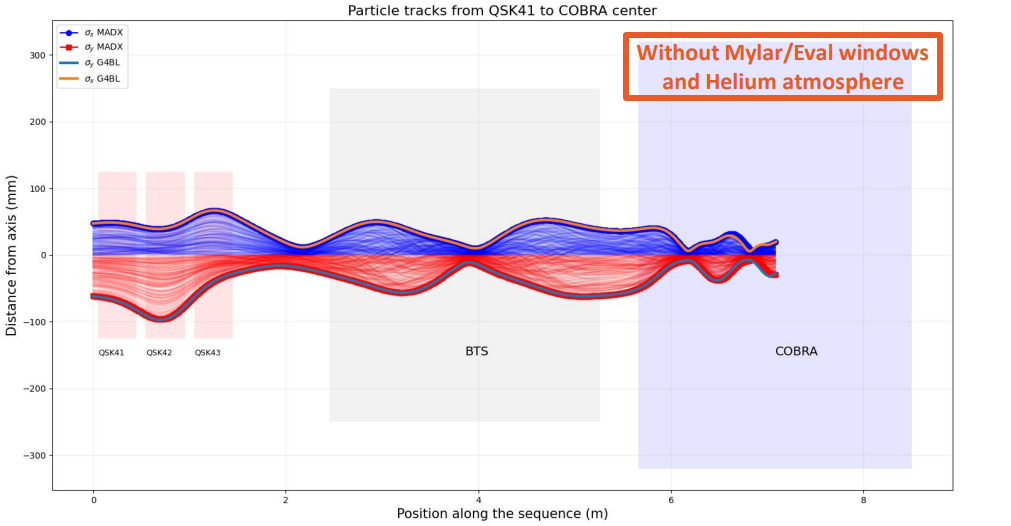
\includegraphics[width = \textwidth]{Figures/MEG/madx_vs_g4b.png}
            \caption{Comperison of the results from the \gfb and \madx simulations for $\pi E5$.}
            \label{fig:madx_vs_g4b}
        \end{figure}
    
    \subsection{MEG II target}
        \paragraph{Deformation and pictures}
        
\section{Cockcroft–Walton}
    In addition to the muon beamline, MEG II has a Cockcroft–Walton proton accelerator. 
    After the description of the machine, we will see the use of this accelerator by the collaboration: calibrations and exotic searches. 

    \subsection{Description of the machine}
        \paragraph{Source}
        \paragraph{Circuit}
        \paragraph{Gas system}
        \paragraph{Controls}

        \begin{figure}
            \centering
            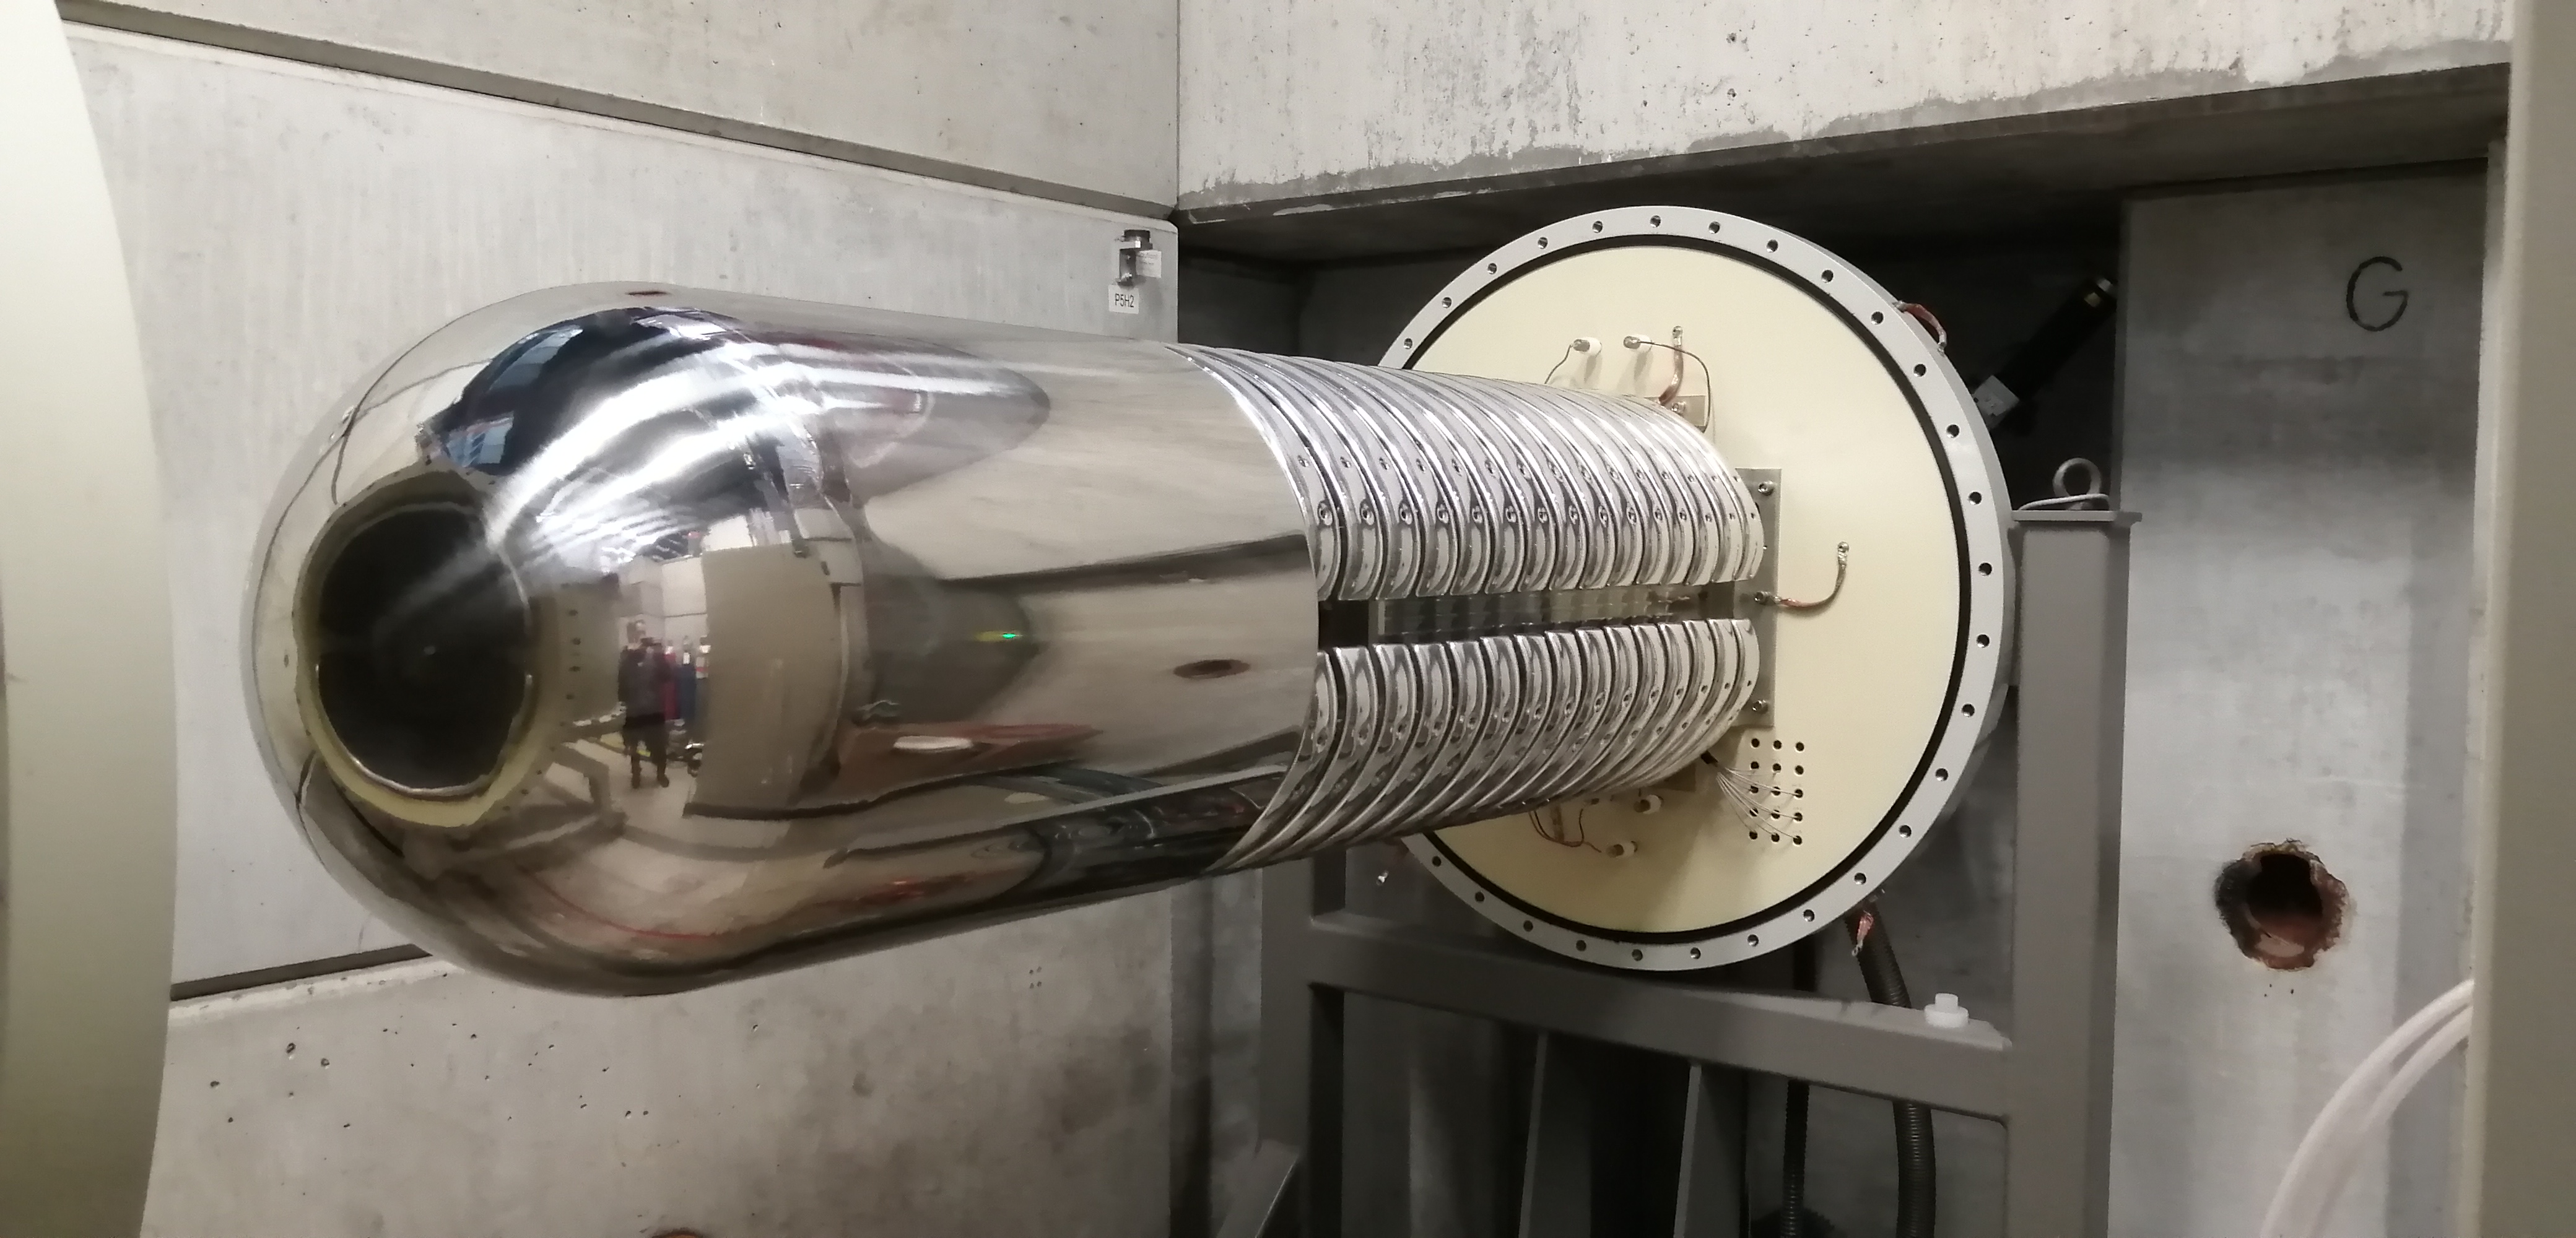
\includegraphics[width=1\textwidth]{Figures/MEG/CW/view_front.jpg}
            %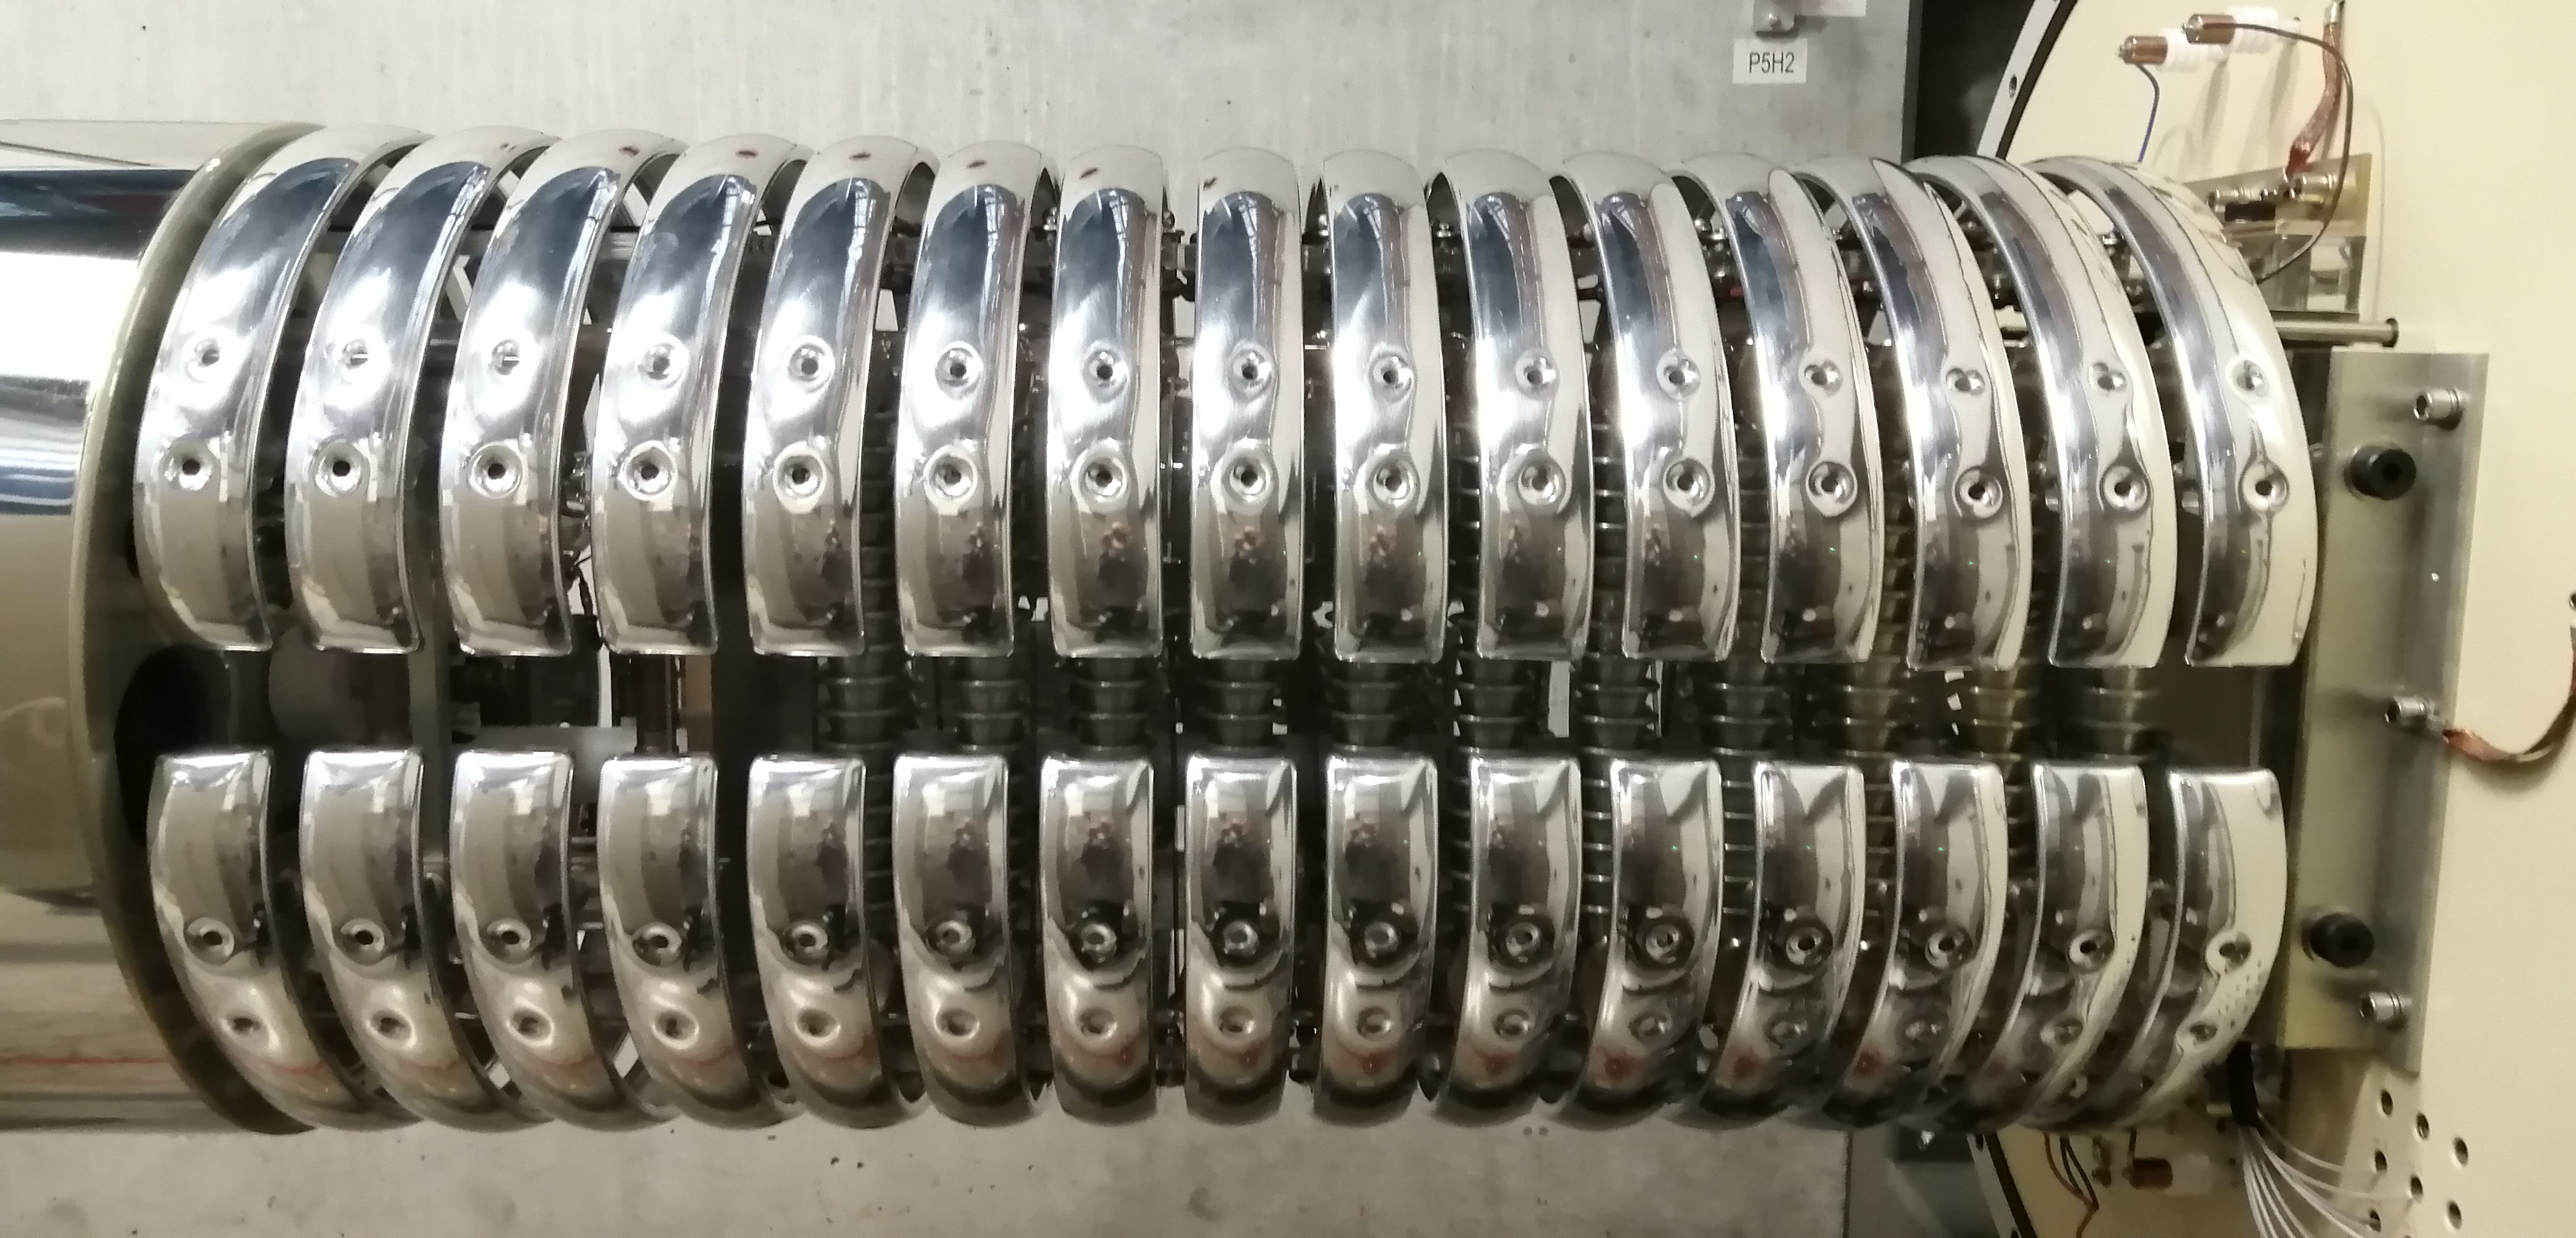
\includegraphics[width=1\textwidth]{Figures/MEG/CW/view_side.jpg}
            \caption{View of the CW after the extraction from the external volume. This volume contains \ce{SF6} which is used as a gaseous dielectric medium and needs to be evacuated before the extraction.}
            \label{fig:CW:view}
            \end{figure}

        \begin{figure}
            \centering
            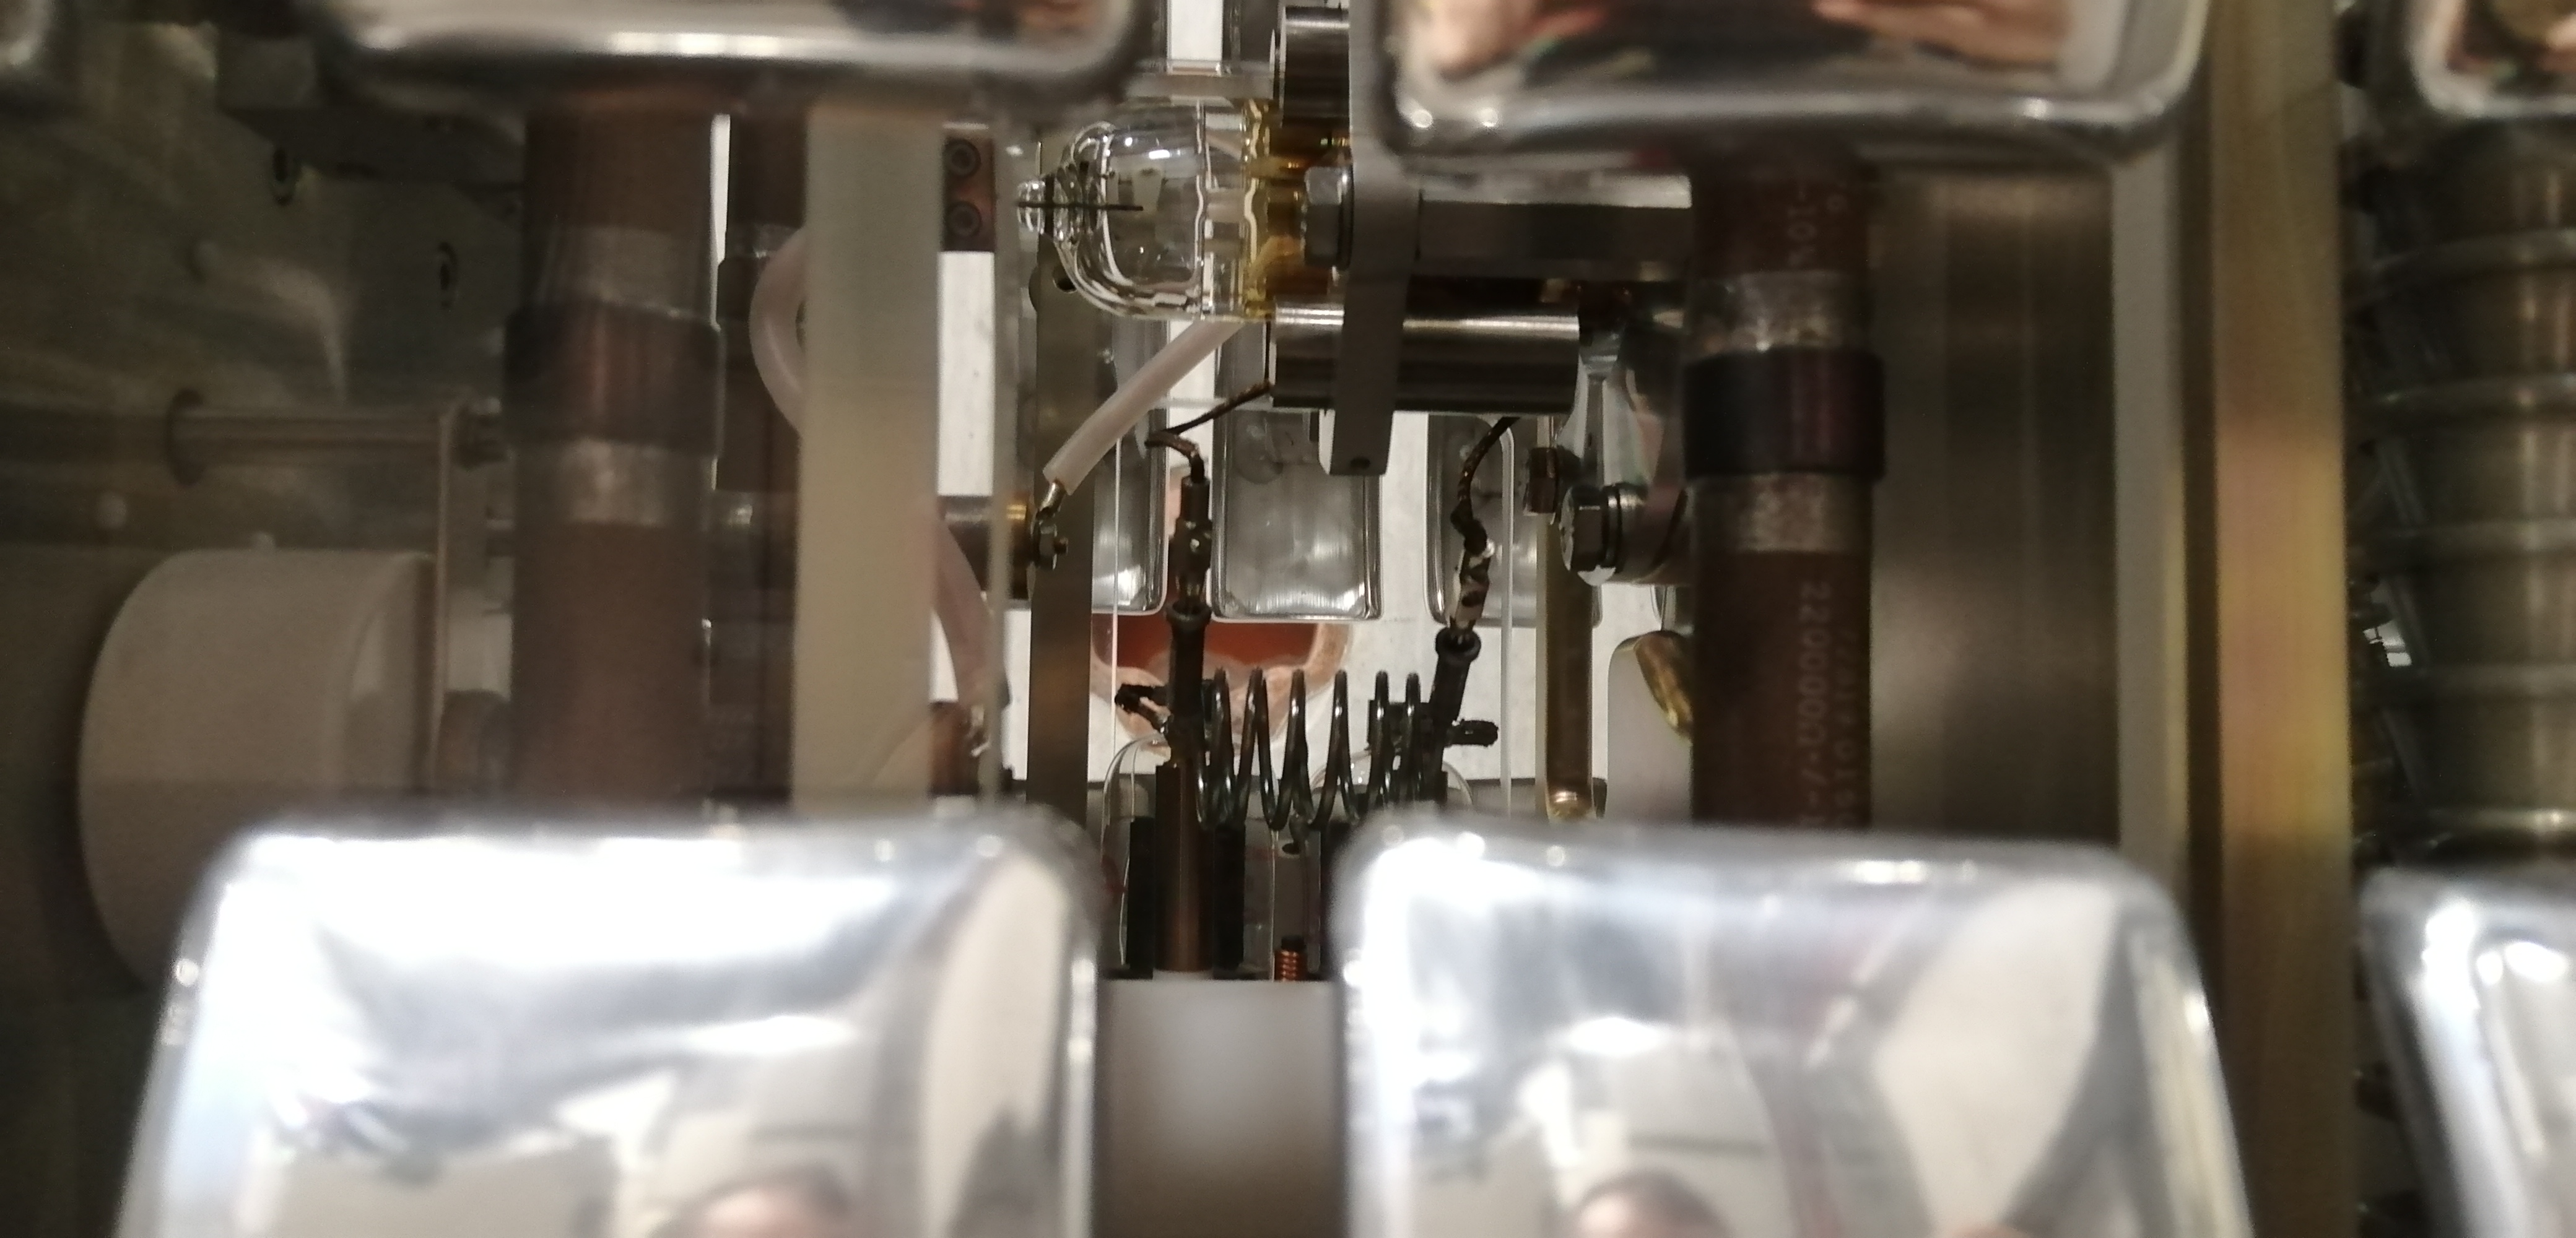
\includegraphics[width=1\textwidth]{Figures/MEG/CW/view_source.jpg}
            \caption{View of the source of the CW   machine.}
            \label{fig:CW:view_source}
        \end{figure}

        \begin{figure}
            \centering
            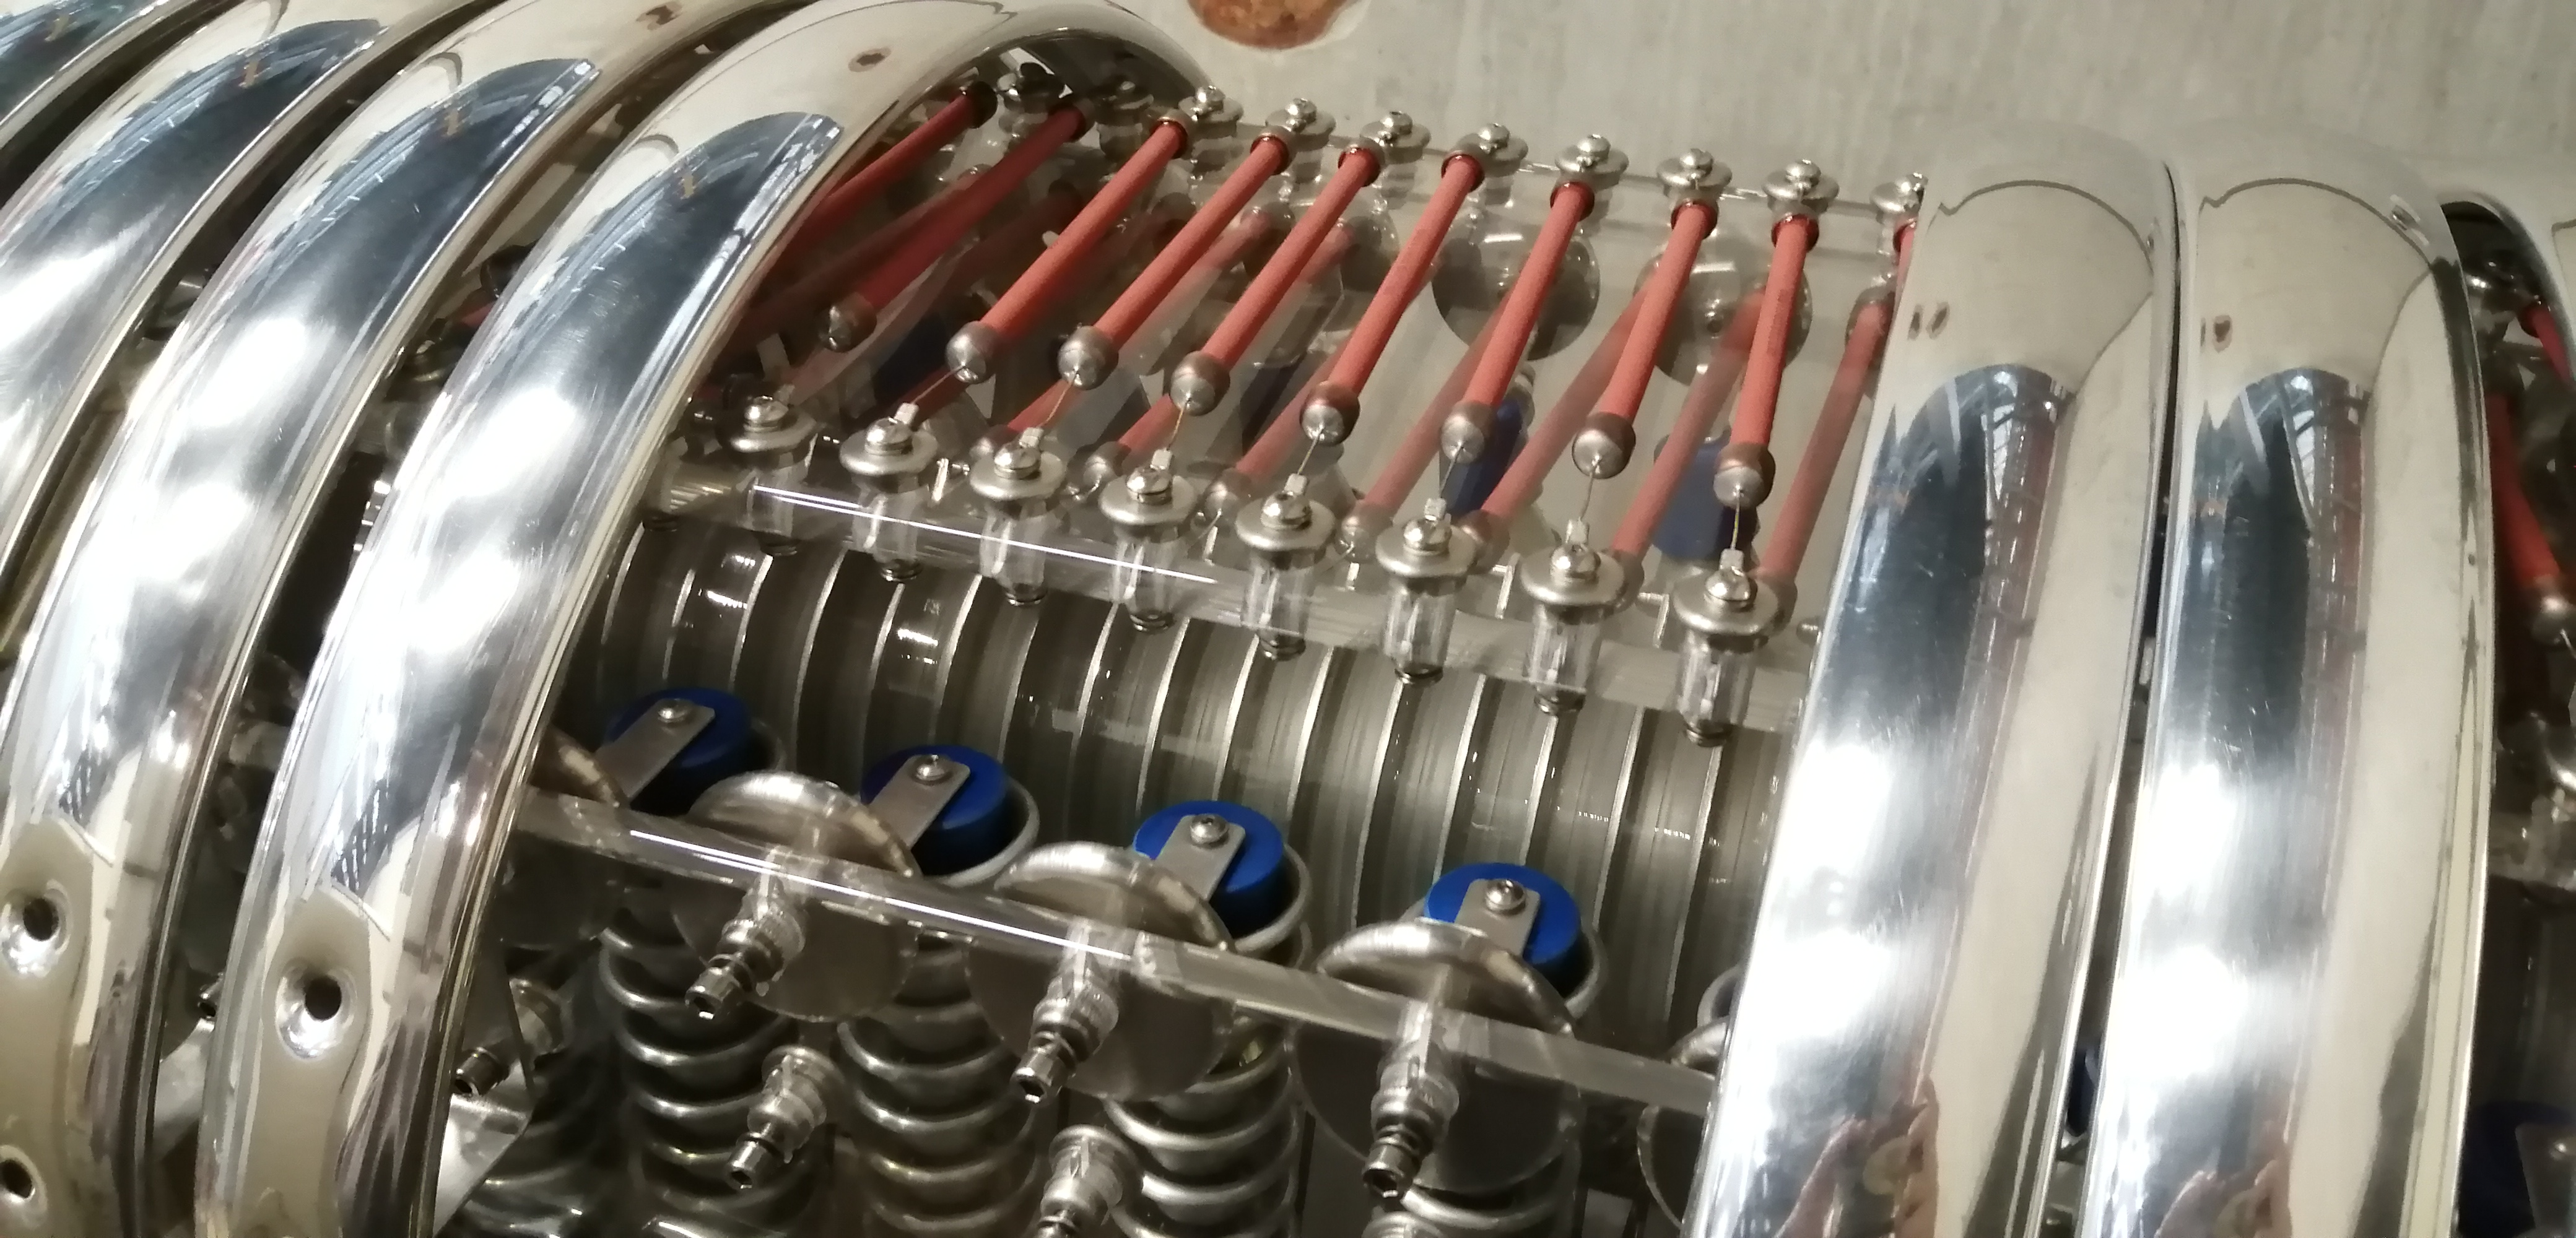
\includegraphics[width=1\textwidth]{Figures/MEG/CW/view_top.jpg}
            \caption{Top view of the CW after the removal of a few AAA. Here we can see all the elements of a CW circuit: red - the resistors on top; metallic rings on the central tube - the capacitors; blue and metallic cups - the resistance and capacitors of the rectifiers, which run vertically.}
            \label{fig:CW:view_top}
        \end{figure}

        \begin{figure}
            \centering
            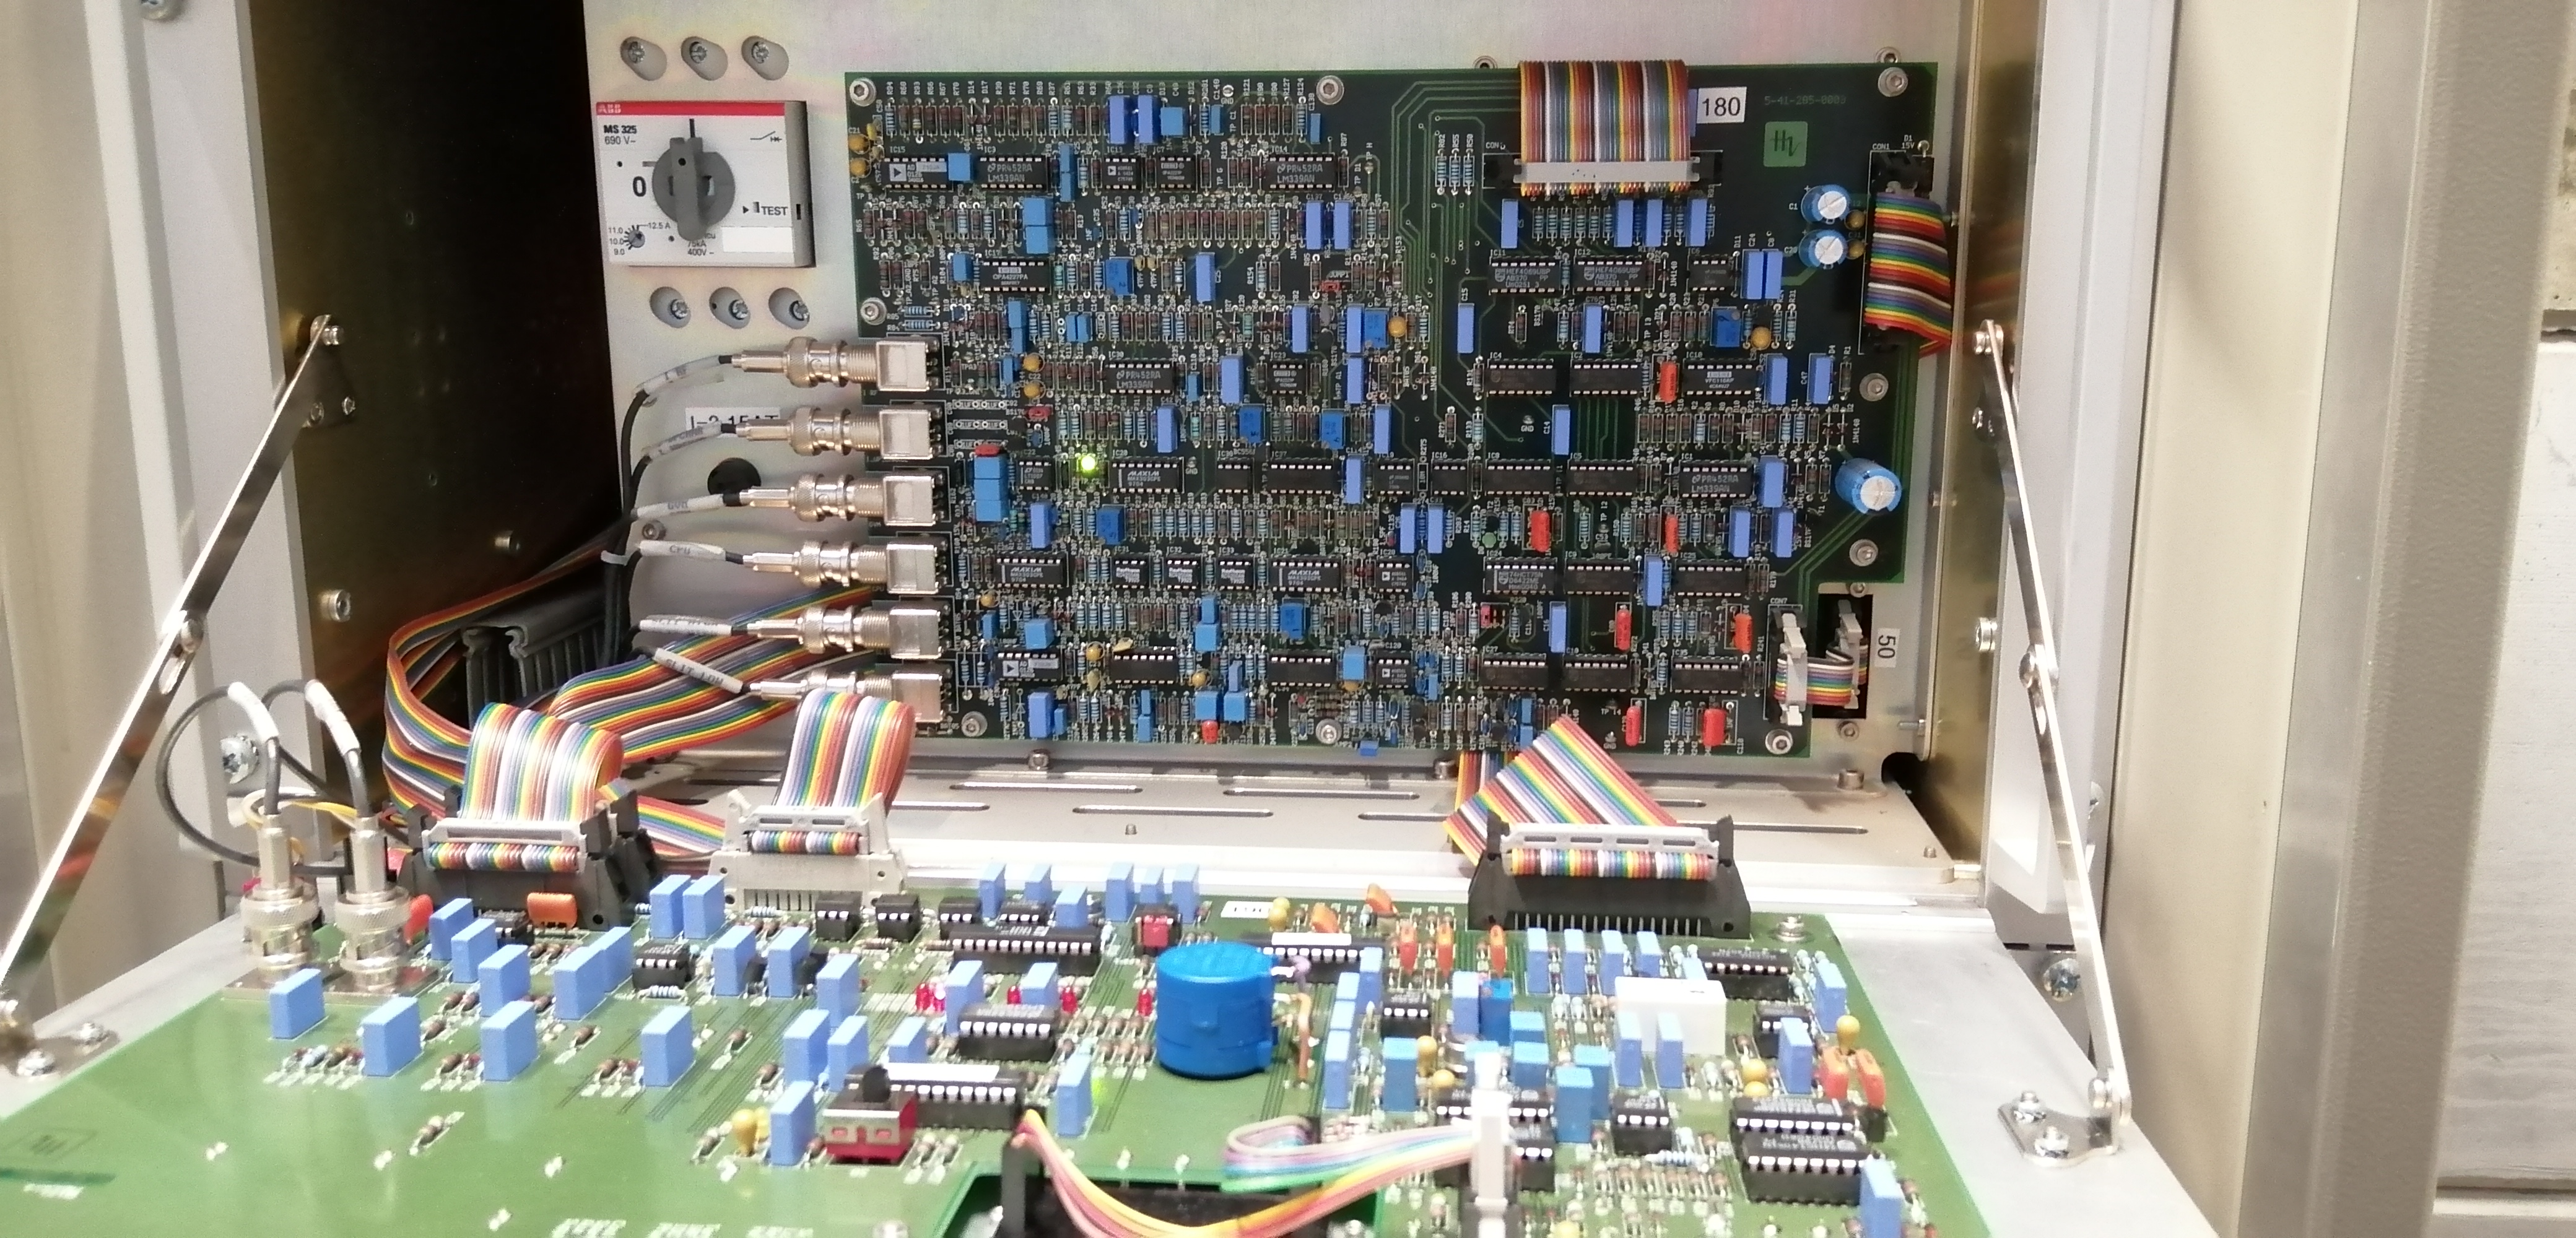
\includegraphics[width=1\textwidth]{Figures/MEG/CW/panel.jpg}
            \caption{Picture of the control panel for the CW machine.}
            \label{fig:CW:panel}
        \end{figure}

    \subsection{XEC calibrations}
        On top of the LED calibration illustrated in \ref{LED} 
        \paragraph{`Standard' lithium calibration}
        \paragraph{Charge EXchange reaction}

    \subsection{X17}
        Although the protons coming from the CW have been mainly used for the calibration of the XEC detector, this machine is also used to perform parasitic measurements.
        The search for the X17 anomaly done in 2021/2022 will be extensively discussed in the dedicated chapter \ref{ch:X17} but we wanted to underline the key role that the CW machine has played in this parasitic search for exotic physics. 

\status{review}
\section{CW issues and maintenance}
    By the end of 2020, the CW started having some minor problems: the machine was running fine but the time required to switch it on kept growing longer. 
    While the whole procedure would normally take $\sim$ 15 min the time required exceeded the hour.
    Following this behavior, an intense exchange with the HV company started and we performed many different tests on both the software and hardware sides.
    In the following period, we also noticed the machine was getting unstable when running near the maximum voltage at \SI{1}{MV}.
    We performed a measurement of the Q-factor of the machine, shown in Fig. \ref{fig:CW:Q-factor}. The value found was a factor $\sim2k$ lower than expected and the position of the resonance frequency was shifted from the design value.
    We adjusted the frequency at which the machine starts when turning ON. 
    This solved the delay problem but didn't recover the maximum voltage. 
    The machine was now starting quickly but working in a stable configuration up to half of the nominal maximum voltage.
    As explained in the previous paragraph this was not a problem for the `usual' calibrations but was a worrying sign on the health of the machine and would have prevented the CEX.
    At this point, an expert from HV was sent to inspect the machine.
    \begin{figure}
        \centering
        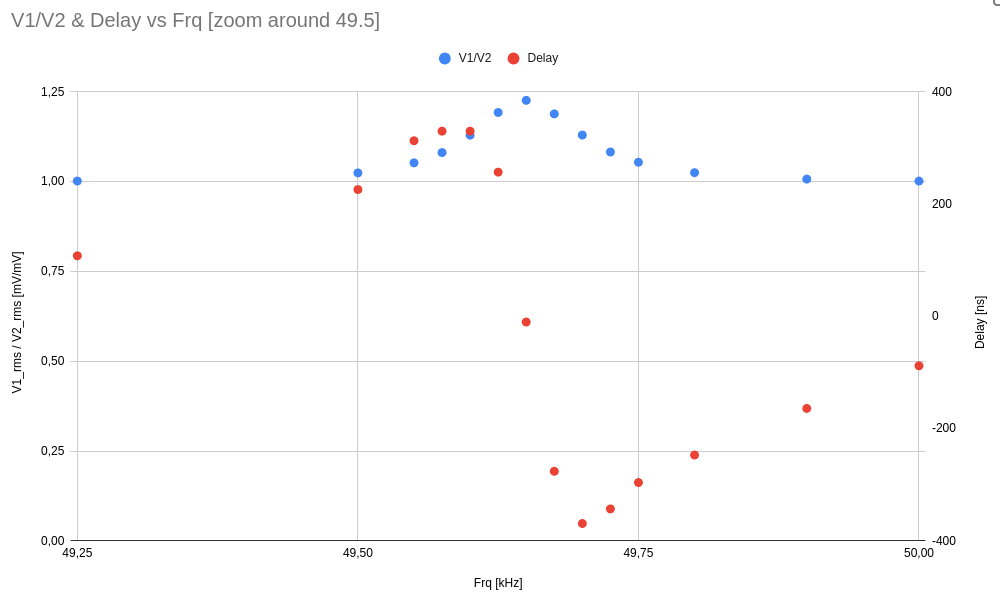
\includegraphics[width=1\textwidth]{Figures/MEG/CW/CW_Q-factor.png}
        \caption{Measurement of the Q-factor}
        \label{fig:CW:Q-factor}
    \end{figure}
    After running some checks opening the CW was deemed necessary and for this reason, we removed the \ce{SF6} contained in the main tank. 
    This gas is often used as a gaseous dielectric medium because of its high dielectric strength, the result of the gas's high electronegativity
    \footnote{Electronegativity is a measure of the attraction of an atom for bonding electrons in molecules compared to that of other atoms: large values indicate a stronger attraction and it increases from left to right across the periodic table.} and density.
    In the case of an arc \ce{SF6} can break down in different ways but most of the decomposition products tend to quickly re-form \ce{SF6}, a process termed \textit{self-healing}. 
    Arcing or corona can also produce disulfur decafluoride (\ce{S2F10}), a highly toxic gas, which is the reason extra care is needed when opening such a system.
    After the extraction of the CW, we inspected and measured all the elements, removing also some of the AAA for easier inspection. 
    We found signs of arcing on one of the rectifiers. 
    After the substitution of this element, the machine was closed again, filled with \ce{SF6}, and tested again.
    This whole process is shown in the pictures in Fig. \ref{fig:CW:broken}.
    Unfortunately, the faulty behavior persisted and we noticed sparks in the main volume. 
    After re-opening we found burning marks on the rectifier next to the exchanged one.
    We then realized that both rectifiers were damaged but the first was functioning as a `bridge', preventing the second from being completely destroyed. 
    After the substitution of the second and the tuning of the machine, we finally recovered its full functionality: quick switching ON and stable operation in the full range of voltages.
    The rectifiers are stacks of alternated diodes and aluminum capacitors capped by two resistors. For both broken elements, we could re-use the capacitors, after careful cleaning, while resistors and diodes were too badly damaged. The process of refurbishing is shown in Fig. \ref{fig:CW:fixed}.

    \begin{figure}[ht]   
        \centering
        \subfloat[Discovery of the burning marks on two rectifiers. The reflectivity was a challenge in taking the picture.]{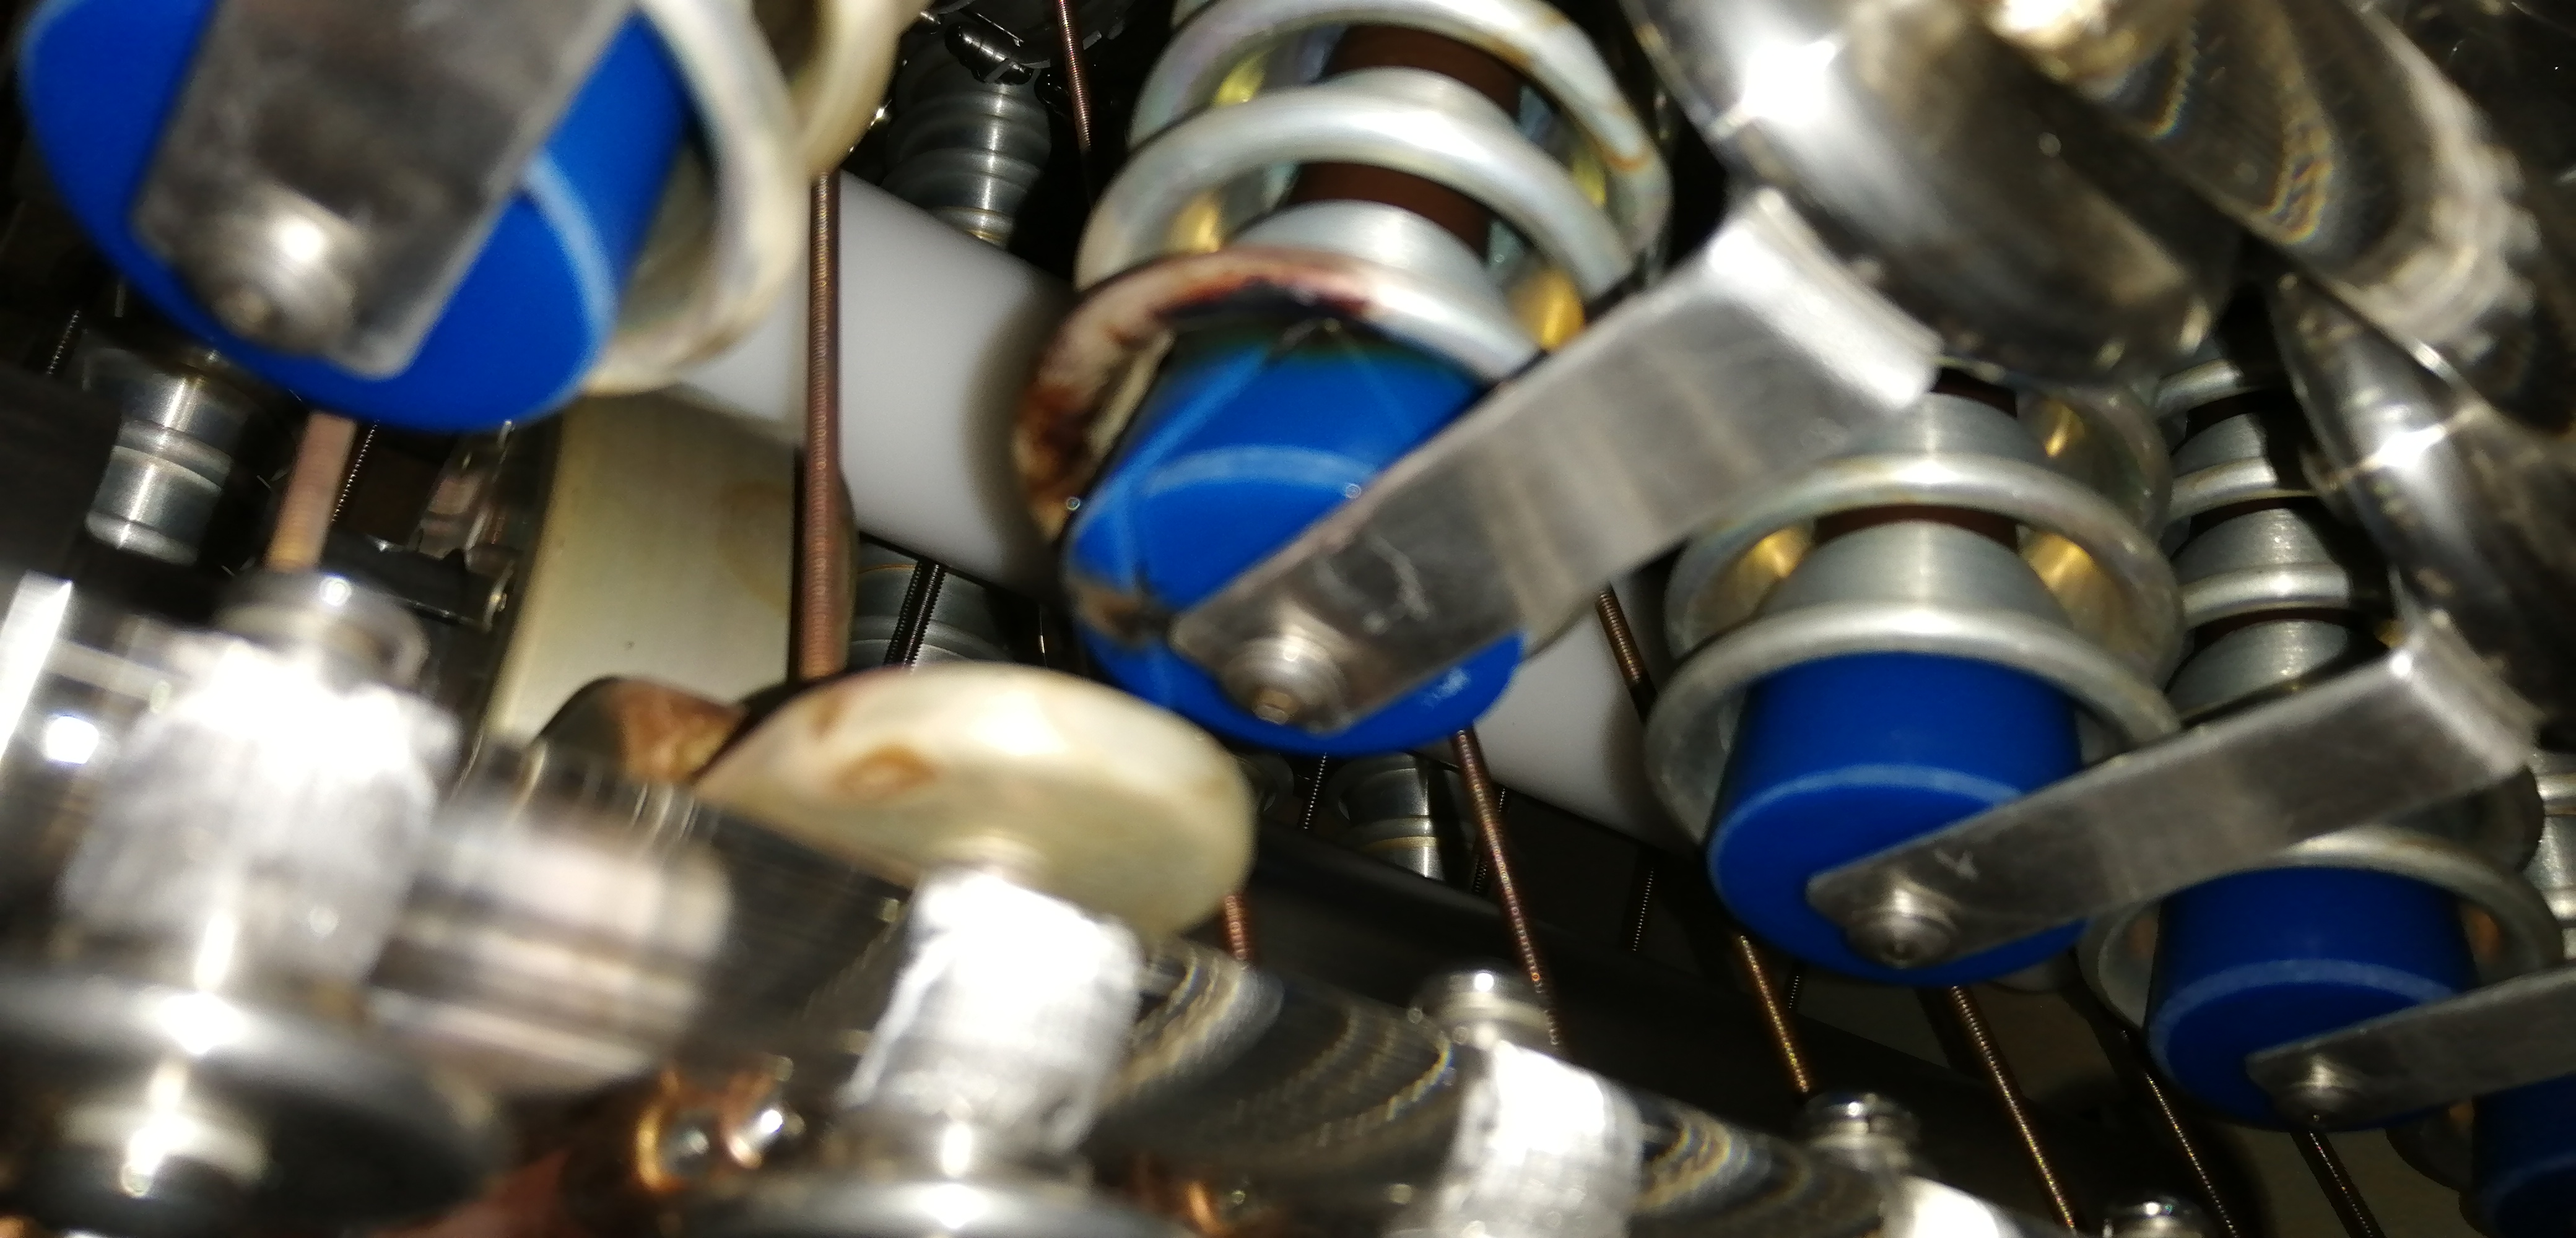
\includegraphics[width=1\textwidth, keepaspectratio]{Figures/MEG/CW/bnurned_in.jpg}\label{fig:CW:burned_in}}\\
        \subfloat[Extraction of the broken rectifiers.]{
        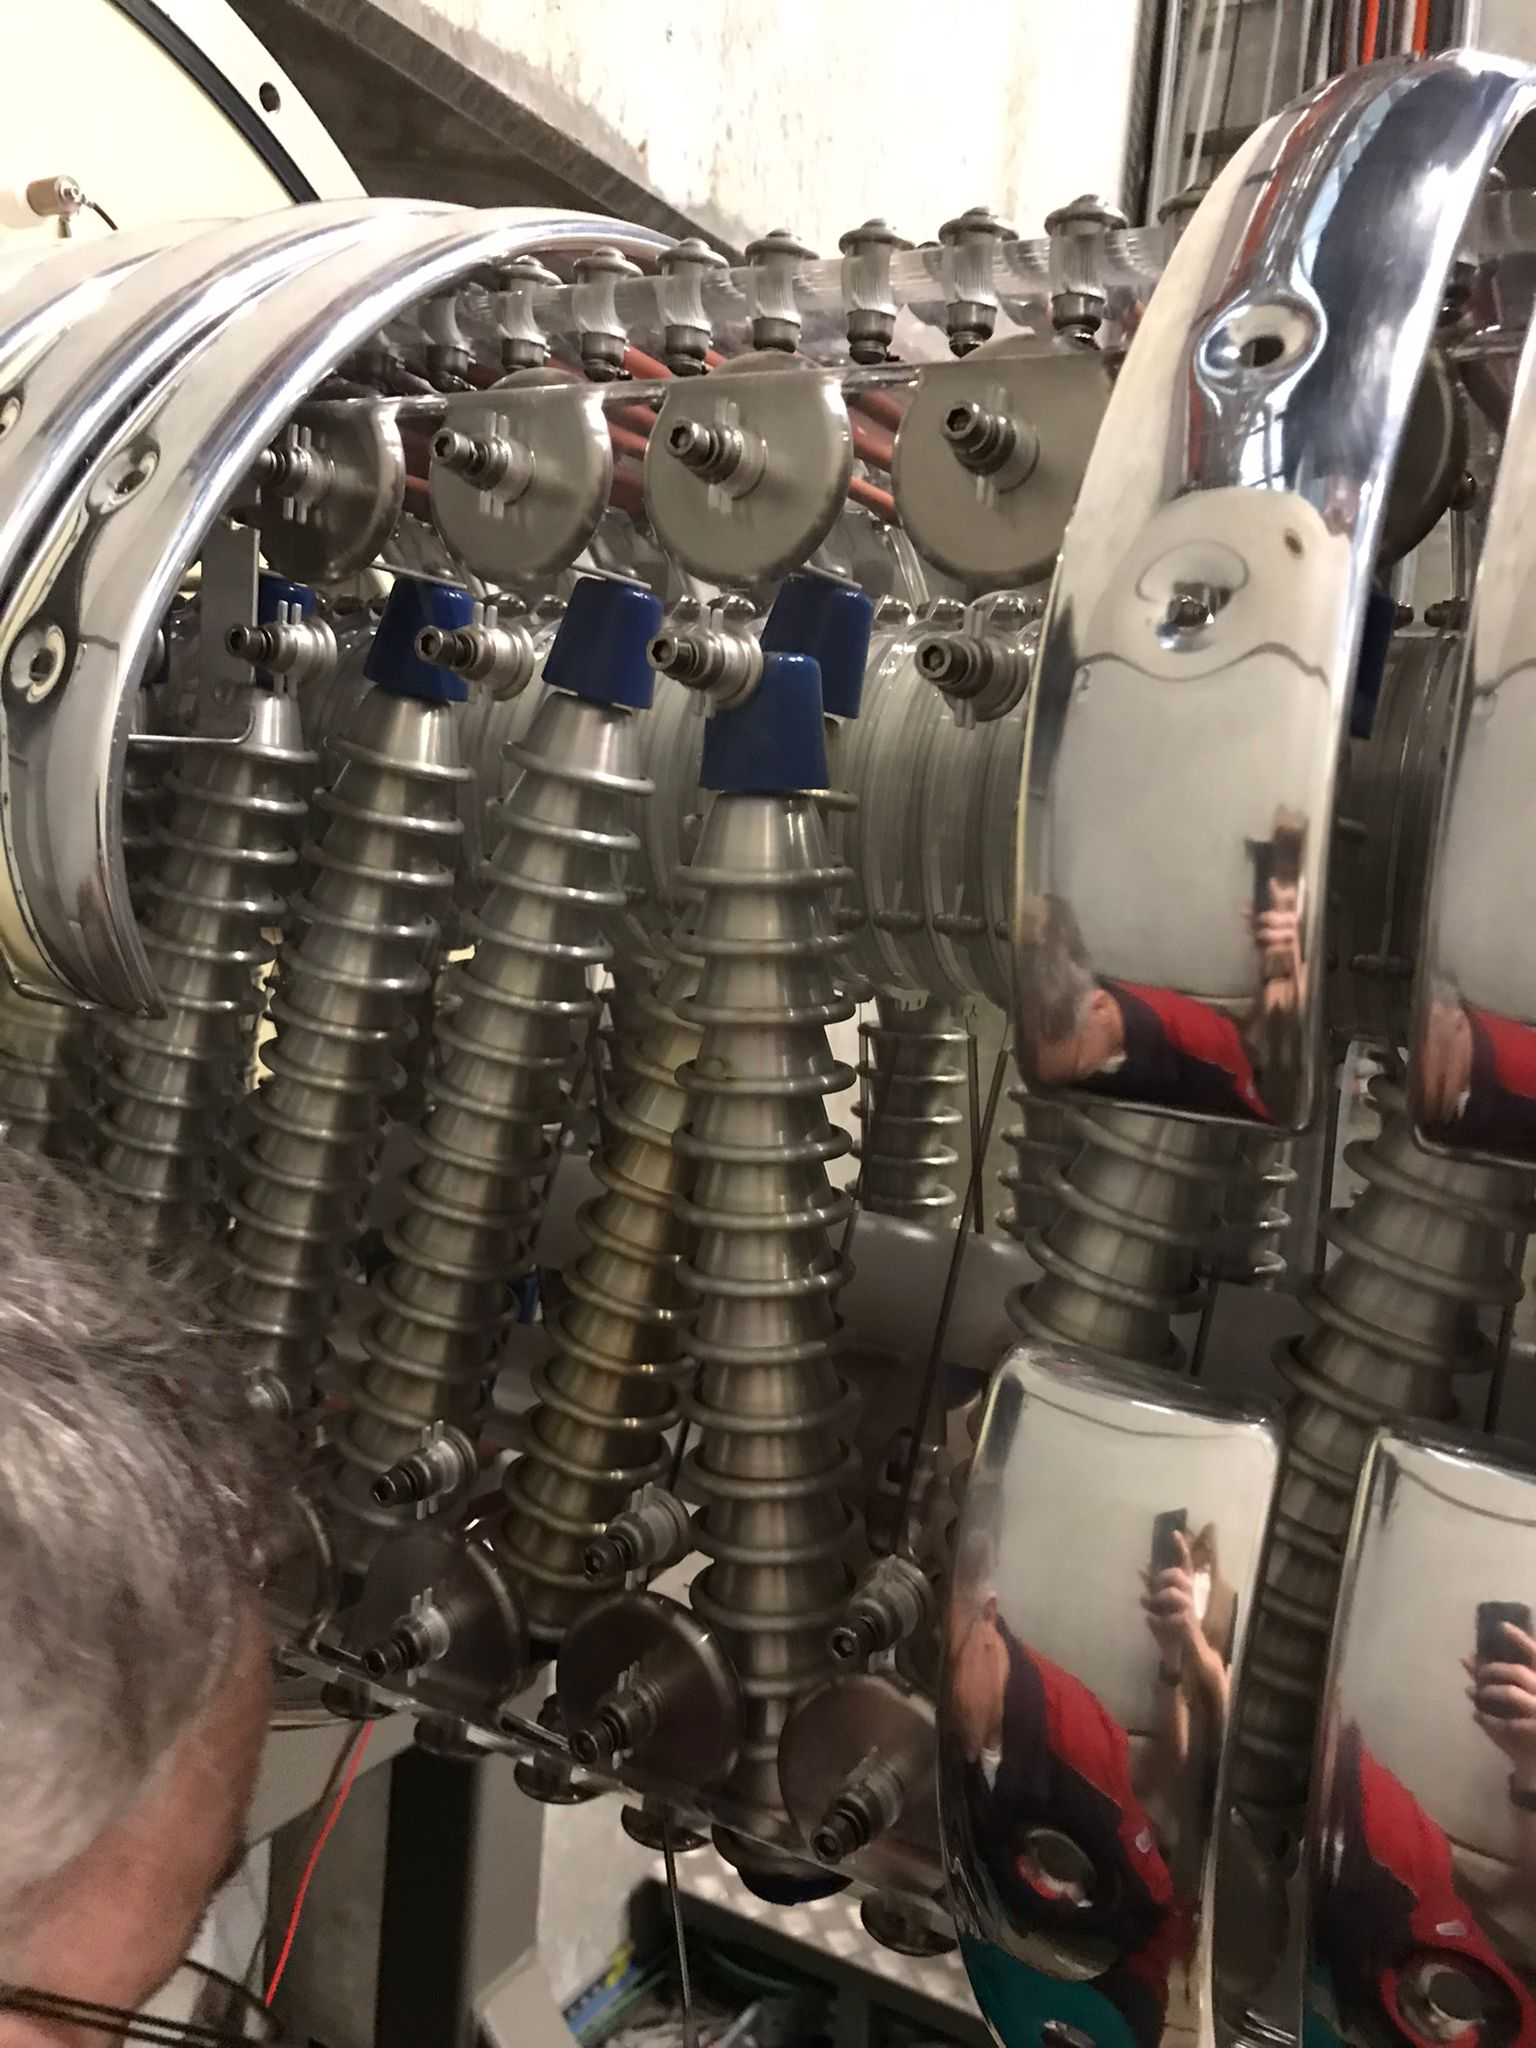
\includegraphics[width=0.49\textwidth, keepaspectratio]{Figures/MEG/CW/removal.jpg}\label{fig:CW:removal}}
        \hfill
        \subfloat[Broken rectifier after the extraction: clearly visible is the burned blue resistor at the top.]{
        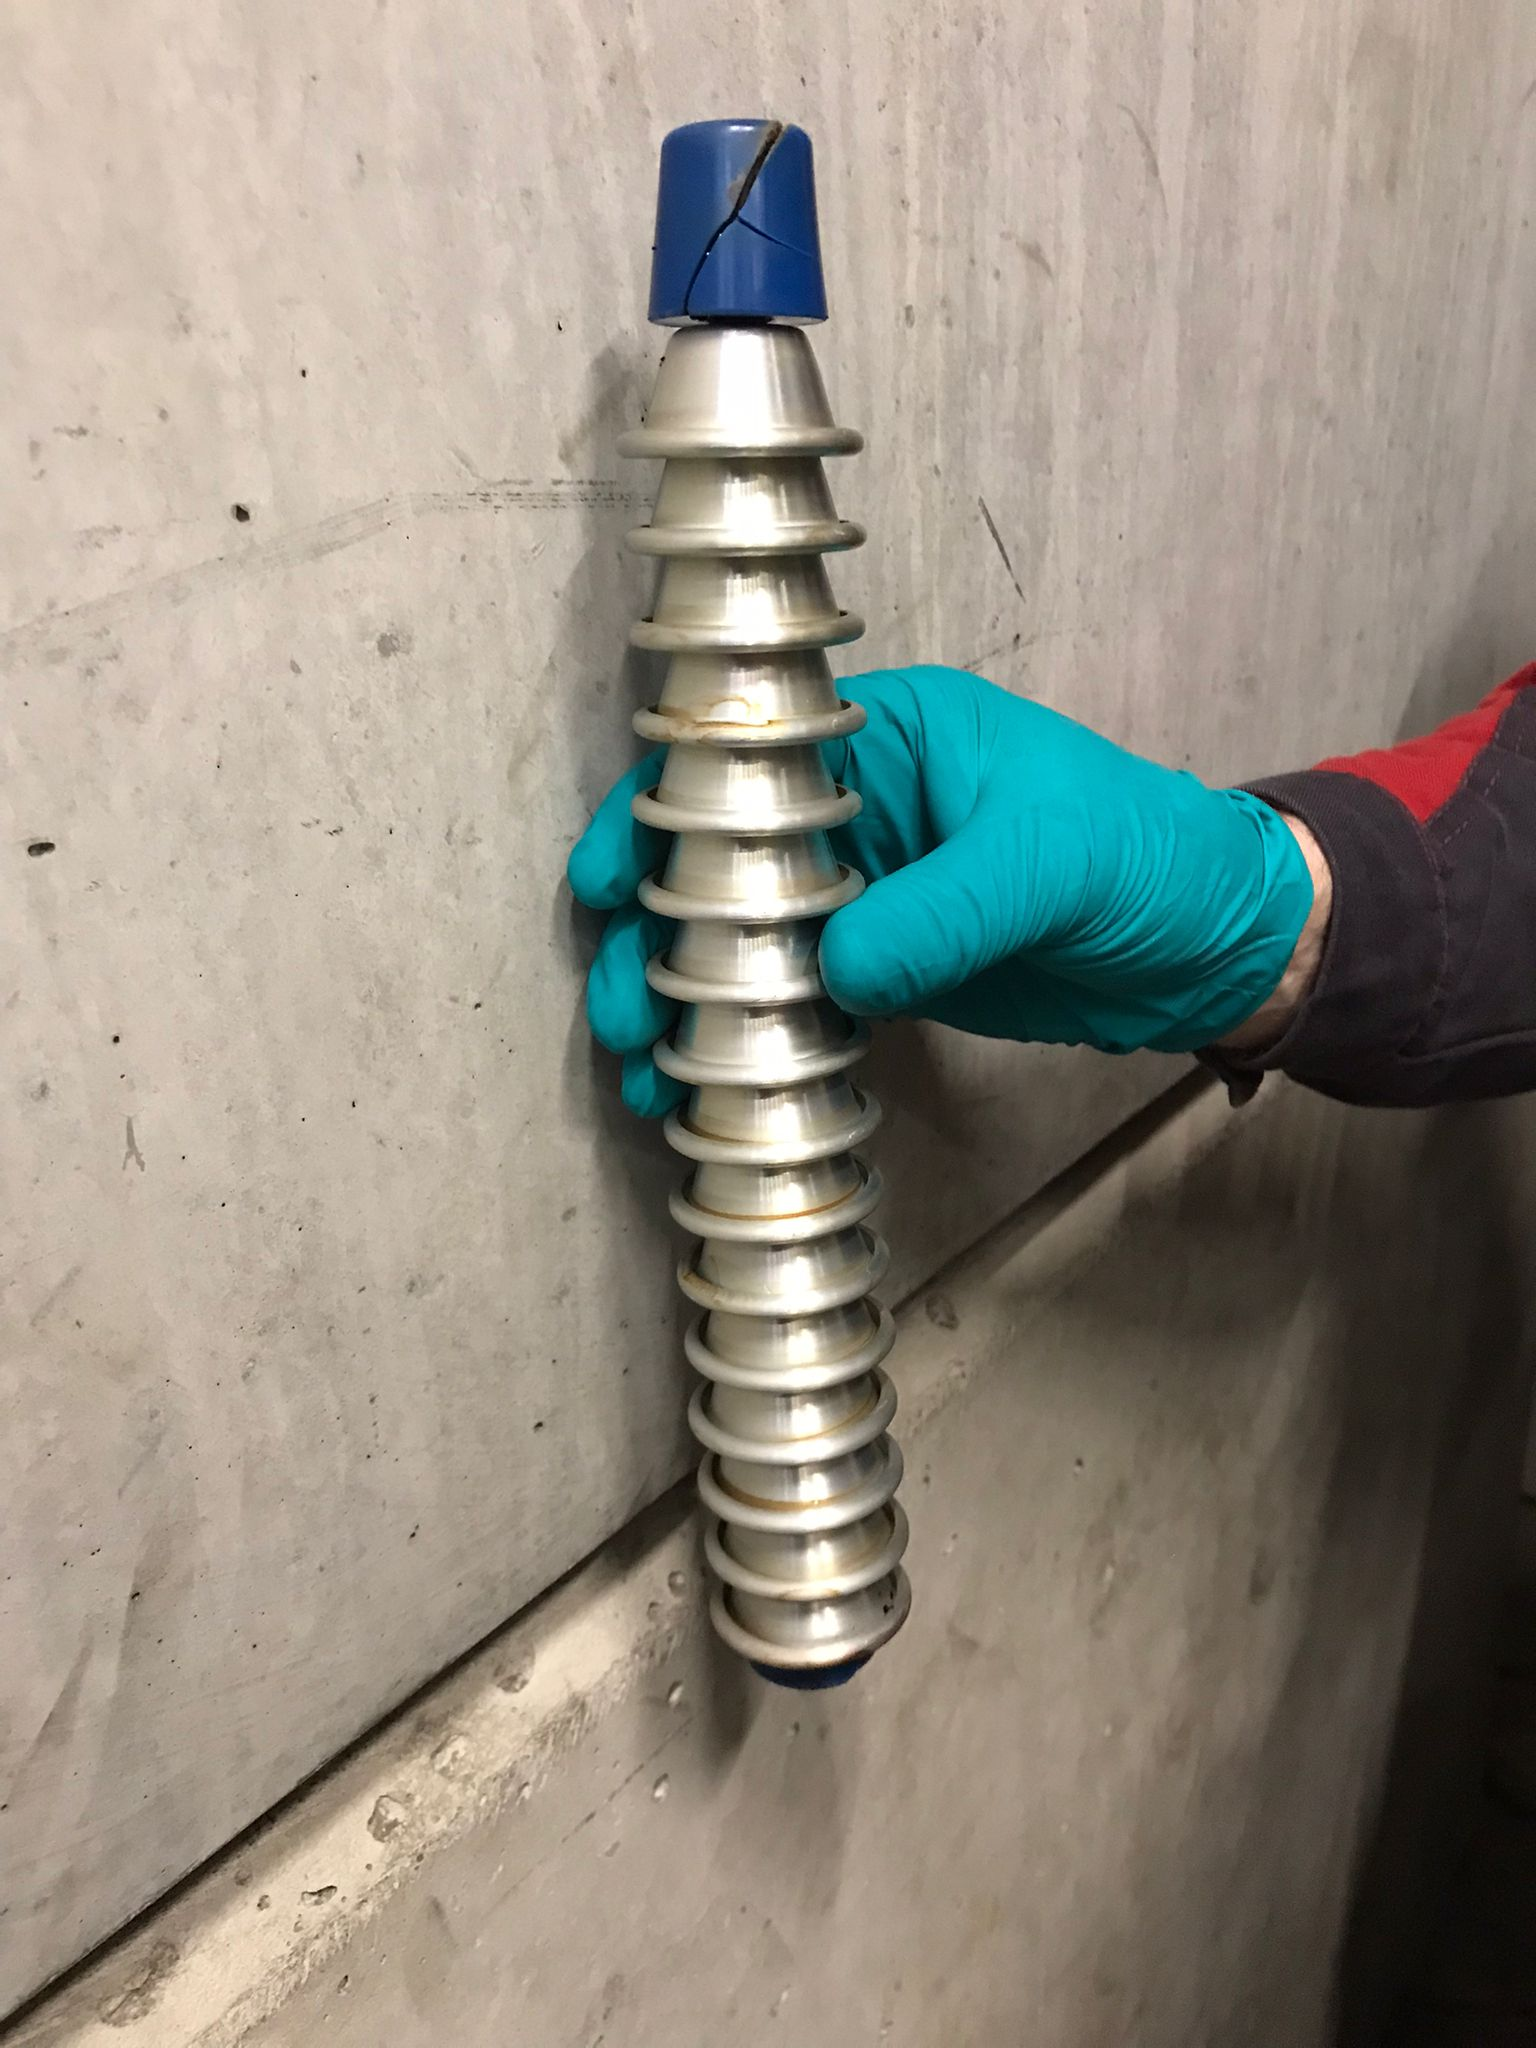
\includegraphics[width=0.49\textwidth, keepaspectratio]{Figures/MEG/CW/rect_broken.jpg}\label{fig:CW:rect_broken}}
        \caption{After close inspection we found burning marks on two rectifiers (\ref{fig:CW:burned_in}). These were removed (\ref{fig:CW:removal}) and carefully inspected (\ref{fig:CW:rect_broken}). The only salvageable part of the rectifiers were the aluminum capacitors, which we cleaned from burning residuals, while all diodes and resistors had to be exchanged.}
        \label{fig:CW:broken}
    \end{figure}

    \begin{figure}[ht]   
        \centering
        \subfloat[Picture of the burning marks on the end resistors of the two rectifiers.]{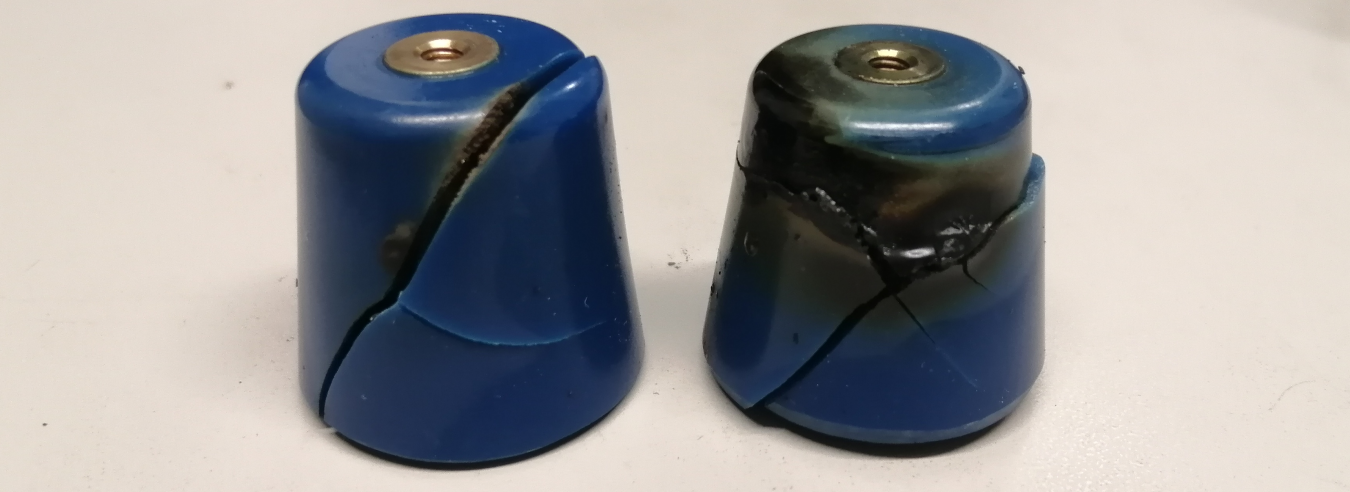
\includegraphics[width=1\textwidth, keepaspectratio]{Figures/MEG/CW/burned.png}\label{fig:CW:burned}}\\
        \subfloat[Assembly of one of the new rectifiers: black - resistors; brown - diodes; metallic - aluminum capacitors.]{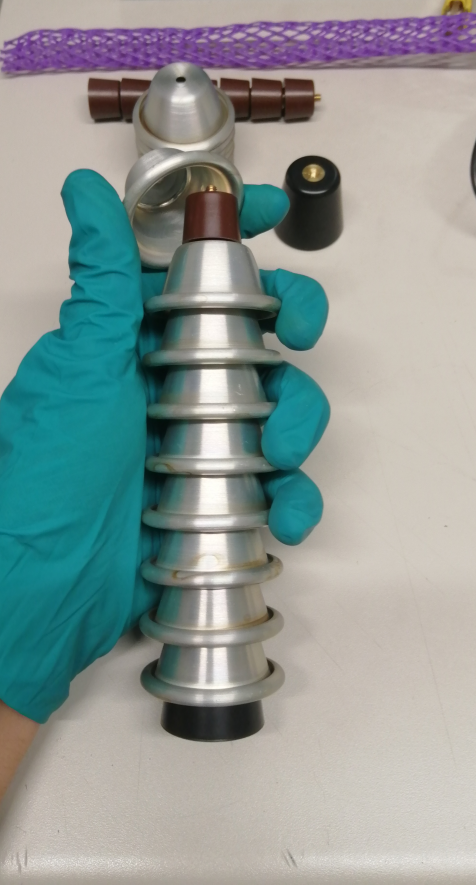
\includegraphics[width=0.49\textwidth]{Figures/MEG/CW/rect_build.png}\label{fig:CW:rect_build}}
        \hfill
        \subfloat[One of the finished new rectifiers.]{
        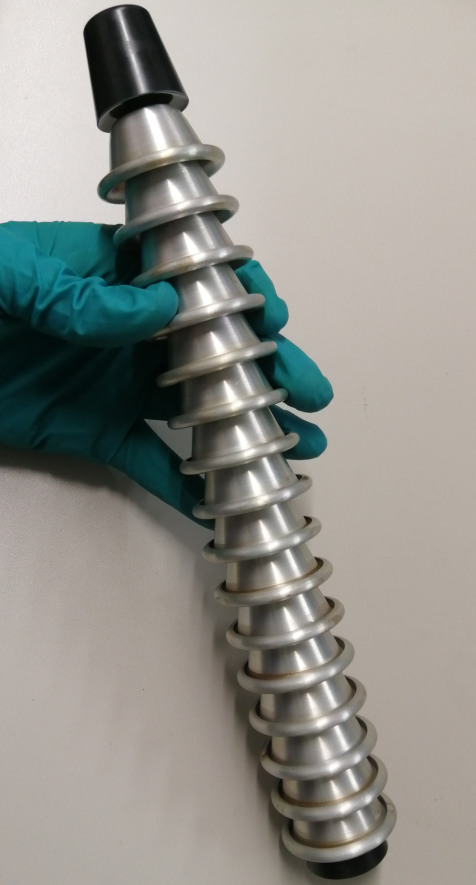
\includegraphics[width=0.49\textwidth, keepaspectratio]{Figures/MEG/CW/rect_new.png}\label{fig:CW:rect_new}}
        \caption{The rectifiers are made of three elements: diodes; aluminum capacitors; resistors (\ref{fig:CW:burned}). Only the capacitors were salvageable: we re-assembled the rectifiers with new diodes and resistors (\ref{fig:CW:rect_build}; \ref{fig:CW:rect_new}).}
        \label{fig:CW:fixed}
    \end{figure}

\section{Conclusions}

\printbibliography[
    heading = bibliographychapter,
    title=Bibliography on MEG II
]

\end{refsection}
